

\tikzset{every picture/.style={line width=0.75pt}} %set default line width to 0.75pt        

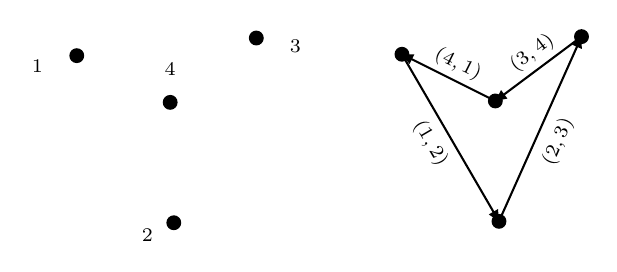
\begin{tikzpicture}[x=0.75pt,y=0.75pt,yscale=-1,xscale=1]
%uncomment if require: \path (0,300); %set diagram left start at 0, and has height of 300

%Shape: Circle [id:dp8468581866061076] 
\draw  [fill={rgb, 255:red, 0; green, 0; blue, 0 }  ,fill opacity=1 ] (129.75,151.67) .. controls (129.75,149.98) and (131.13,148.6) .. (132.83,148.6) .. controls (134.52,148.6) and (135.9,149.98) .. (135.9,151.67) .. controls (135.9,153.37) and (134.52,154.75) .. (132.83,154.75) .. controls (131.13,154.75) and (129.75,153.37) .. (129.75,151.67) -- cycle ;
%Shape: Circle [id:dp1092279369277932] 
\draw  [fill={rgb, 255:red, 0; green, 0; blue, 0 }  ,fill opacity=1 ] (131.5,209.67) .. controls (131.5,207.98) and (132.88,206.6) .. (134.58,206.6) .. controls (136.27,206.6) and (137.65,207.98) .. (137.65,209.67) .. controls (137.65,211.37) and (136.27,212.75) .. (134.58,212.75) .. controls (132.88,212.75) and (131.5,211.37) .. (131.5,209.67) -- cycle ;
%Shape: Circle [id:dp47847609424251114] 
\draw  [fill={rgb, 255:red, 0; green, 0; blue, 0 }  ,fill opacity=1 ] (171.25,120.67) .. controls (171.25,118.98) and (172.63,117.6) .. (174.33,117.6) .. controls (176.02,117.6) and (177.4,118.98) .. (177.4,120.67) .. controls (177.4,122.37) and (176.02,123.75) .. (174.33,123.75) .. controls (172.63,123.75) and (171.25,122.37) .. (171.25,120.67) -- cycle ;
%Shape: Circle [id:dp13281179663837128] 
\draw  [fill={rgb, 255:red, 0; green, 0; blue, 0 }  ,fill opacity=1 ] (84.75,129.17) .. controls (84.75,127.48) and (86.13,126.1) .. (87.83,126.1) .. controls (89.52,126.1) and (90.9,127.48) .. (90.9,129.17) .. controls (90.9,130.87) and (89.52,132.25) .. (87.83,132.25) .. controls (86.13,132.25) and (84.75,130.87) .. (84.75,129.17) -- cycle ;
%Shape: Circle [id:dp9047785488054659] 
\draw  [fill={rgb, 255:red, 0; green, 0; blue, 0 }  ,fill opacity=1 ] (286.42,151.01) .. controls (286.42,149.31) and (287.79,147.93) .. (289.49,147.93) .. controls (291.19,147.93) and (292.57,149.31) .. (292.57,151.01) .. controls (292.57,152.71) and (291.19,154.08) .. (289.49,154.08) .. controls (287.79,154.08) and (286.42,152.71) .. (286.42,151.01) -- cycle ;
%Shape: Circle [id:dp4512249144398415] 
\draw  [fill={rgb, 255:red, 0; green, 0; blue, 0 }  ,fill opacity=1 ] (288.17,209.01) .. controls (288.17,207.31) and (289.54,205.93) .. (291.24,205.93) .. controls (292.94,205.93) and (294.32,207.31) .. (294.32,209.01) .. controls (294.32,210.71) and (292.94,212.08) .. (291.24,212.08) .. controls (289.54,212.08) and (288.17,210.71) .. (288.17,209.01) -- cycle ;
%Shape: Circle [id:dp7255085919283367] 
\draw  [fill={rgb, 255:red, 0; green, 0; blue, 0 }  ,fill opacity=1 ] (327.92,120.01) .. controls (327.92,118.31) and (329.29,116.93) .. (330.99,116.93) .. controls (332.69,116.93) and (334.07,118.31) .. (334.07,120.01) .. controls (334.07,121.71) and (332.69,123.08) .. (330.99,123.08) .. controls (329.29,123.08) and (327.92,121.71) .. (327.92,120.01) -- cycle ;
%Shape: Circle [id:dp7940275676020767] 
\draw  [fill={rgb, 255:red, 0; green, 0; blue, 0 }  ,fill opacity=1 ] (241.42,128.51) .. controls (241.42,126.81) and (242.79,125.43) .. (244.49,125.43) .. controls (246.19,125.43) and (247.57,126.81) .. (247.57,128.51) .. controls (247.57,130.21) and (246.19,131.58) .. (244.49,131.58) .. controls (242.79,131.58) and (241.42,130.21) .. (241.42,128.51) -- cycle ;
%Straight Lines [id:da7630243708026373] 
\draw    (244.49,128.51) -- (289.74,206.41) ;
\draw [shift={(291.24,209.01)}, rotate = 239.85] [fill={rgb, 255:red, 0; green, 0; blue, 0 }  ][line width=0.08]  [draw opacity=0] (5.36,-2.57) -- (0,0) -- (5.36,2.57) -- cycle    ;
%Straight Lines [id:da7466547663908568] 
\draw    (291.24,209.01) -- (329.77,122.75) ;
\draw [shift={(330.99,120.01)}, rotate = 114.07] [fill={rgb, 255:red, 0; green, 0; blue, 0 }  ][line width=0.08]  [draw opacity=0] (5.36,-2.57) -- (0,0) -- (5.36,2.57) -- cycle    ;
%Straight Lines [id:da5263162246336347] 
\draw    (330.99,120.01) -- (291.9,149.21) ;
\draw [shift={(289.49,151.01)}, rotate = 323.24] [fill={rgb, 255:red, 0; green, 0; blue, 0 }  ][line width=0.08]  [draw opacity=0] (5.36,-2.57) -- (0,0) -- (5.36,2.57) -- cycle    ;
%Straight Lines [id:da700113901084908] 
\draw    (289.49,151.01) -- (247.17,129.85) ;
\draw [shift={(244.49,128.51)}, rotate = 26.57] [fill={rgb, 255:red, 0; green, 0; blue, 0 }  ][line width=0.08]  [draw opacity=0] (5.36,-2.57) -- (0,0) -- (5.36,2.57) -- cycle    ;

% Text Node
\draw (64.67,129.6) node [anchor=north west][inner sep=0.75pt]  [font=\scriptsize] [align=left] {$\displaystyle 1$};
% Text Node
\draw (117.67,211.27) node [anchor=north west][inner sep=0.75pt]  [font=\scriptsize] [align=left] {$\displaystyle 2$};
% Text Node
\draw (189,120.27) node [anchor=north west][inner sep=0.75pt]  [font=\scriptsize] [align=left] {$\displaystyle 3$};
% Text Node
\draw (128.67,131.27) node [anchor=north west][inner sep=0.75pt]  [font=\scriptsize] [align=left] {$\displaystyle 4$};
% Text Node
\draw (256.73,156.68) node [anchor=north west][inner sep=0.75pt]  [font=\scriptsize,rotate=-59.54] [align=left] {$\displaystyle ( 1,2)$};
% Text Node
\draw (308.71,180.59) node [anchor=north west][inner sep=0.75pt]  [font=\scriptsize,rotate=-293.67] [align=left] {$\displaystyle ( 2,3)$};
% Text Node
\draw (292.72,131.06) node [anchor=north west][inner sep=0.75pt]  [font=\scriptsize,rotate=-323.41] [align=left] {$\displaystyle ( 3,4)$};
% Text Node
\draw (262.25,121.79) node [anchor=north west][inner sep=0.75pt]  [font=\scriptsize,rotate=-26.71] [align=left] {$\displaystyle ( 4,1)$};


\end{tikzpicture}
